\begin{enumerate}

%%%%%%%%% Problem 1 %%%%%%%%%%%
\item Add a table-level PRIMARY KEY constraint to the EMP table on the ID column. The constraint
should be named at creation. Name the constraint \texttt{my\_emp\_id\_pk}.\\
\textbf{Hint: }The constraint is enabled as soon as the ALTER TABLE command executes
successfully.

\textbf{Solution: }
\begin{lstlisting}[language=SQL]
ALTER TABLE emp
ADD CONSTRAINT my_emp_id_pk PRIMARY KEY (id);
\end{lstlisting}
\textbf{Output: }
% \begin{figure}[h]
%     \centering
%     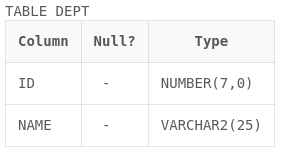
\includegraphics[width=0.5\linewidth]{graphics/p91.png}
% \end{figure}

%%%%%%%%% Problem 2 %%%%%%%%%%%
\item Create a PRIMARY KEY constraint to the DEPT table using the ID column. The constraint should
be named at creation. Name the constraint \texttt{my\_deptid\_pk}.\\
\textbf{Hint: }The constraint is enabled as soon as the ALTER TABLE command executes
successfully.

\textbf{Solution: }
\begin{lstlisting}[language=SQL]
ALTER TABLE dept
ADD CONSTRAINT my_deptid_pk PRIMARY KEY(id);
\end{lstlisting}

%%%%%%%%% Problem 3 %%%%%%%%%%%
\item Add a column \texttt{DEPT\_ID} to the EMP table. Add a foreign key reference on the EMP table that
ensures that the employee is not assigned to a nonexistent department. Name the constraint
\texttt{my\_emp\_dept\_id\_fk}.

\textbf{Solution: }
\begin{lstlisting}[language=SQL]
ALTER TABLE emp
ADD (dept_id NUMBER(7));
ALTER TABLE emp
ADD CONSTRAINT my_emp_dept_id_fk
FOREIGN KEY (dept_id) REFERENCES dept(id);
\end{lstlisting}
% \textbf{Output: }
% \begin{figure}[h]
%     \centering
%     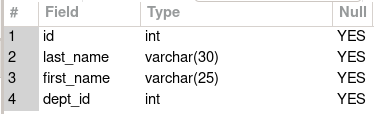
\includegraphics[width=0.5\linewidth]{graphics/p93.png}
% \end{figure}

%%%%%%%%% Problem 4 %%%%%%%%%%%
\item Confirm that the constraints were added by querying the \texttt{USER\_CONSTRAINTS} view. Note the
types and names of the constraints. Save your statement text in a file called \texttt{lab10\_4.sql}.
\begin{figure}[h]
\centering
    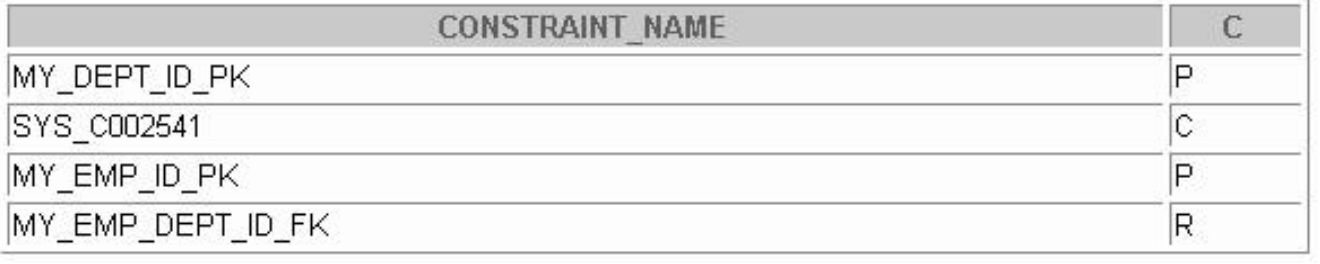
\includegraphics[width=.8\linewidth]{graphics/104.png}
\end{figure}

\textbf{Solution: }
\begin{lstlisting}[language=SQL]
select constraint_name, constraint_type
from user_constraints
where table_name IN ('EMP', 'DEPT');
\end{lstlisting}
\newpage
\textbf{Output: }
\begin{figure}[h]
    \centering
    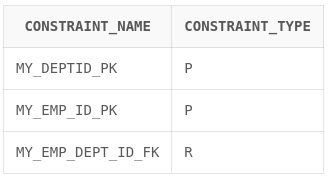
\includegraphics[width=0.5\linewidth]{graphics/p104.png}
\end{figure}

%%%%%%%%% Problem 5 %%%%%%%%%%%

\item Display the object names and types from the \texttt{USER\_OBJECTS} data dictionary view for the EMP
and DEPT tables. Notice that the new tables and a new index were created.

\textbf{Solution: }
\begin{lstlisting}[language=SQL]
SELECT OBJECT_NAME, OBJECT_TYPE
FROM USER_OBJECTS
WHERE OBJECT_NAME IN ('EMP', 'DEPT');
\end{lstlisting}
\textbf{Output: }
\begin{figure}[h]
    \centering
    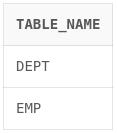
\includegraphics[width=0.3\linewidth]{graphics/p95.png}
\end{figure}

%%%%%%%%% Problem 6 %%%%%%%%%%%
\item Modify the EMP table. Add a COMMISSION column of NUMBER data type, precision 2, scale 2.
Add a constraint to the commission column that ensures that a commission value is greater than
zero.

\textbf{Solution: }
\begin{lstlisting}[language=SQL]
ALTER TABLE emp
ADD commission NUMBER(2, 2);

ALTER TABLE emp
ADD CONSTRAINT chk_commission_positive 
    CHECK (COMMISSION > 0);
\end{lstlisting}

\end{enumerate}

